\section{Design Phase} \label{designPhase}

\subsection{Third Party Libraries}

\begin{multicols}{2}
	\paragraph{Cinder \cite{developers_davis}} \textit{Cinder} is a free, open source graphics engine for \CC. It provides a simple way to access OpenGL, ImGui and other tools, such as image loading and saving, optimised rendering in 2D and 3D, and more. I am using \textit{Cinder} for this project instead of doing all the graphics processing with raw OpenGL because it dramatically simplifies the code, and reduces the scope for hard-to-fix bugs.
	
	Furthermore, I am using a custom fork of the library with my own changes applied to the code, fixing some issues with it and adding some more functionality.
	
	\paragraph{LibRapid \cite{Davis_LibRapid_Optimised_Mathematics_2023}} \textit{LibRapid} is a high-performance library for mathematical applications, including optimised vector classes, complex number types and general mathematical functions. The most useful feature for this project, however, is its support for MPIR and MPFR, which are multiprecision implementations.
	
	Being able to incorporate an efficient multiprecision implementation into the project could allow for ``infinite'' fractal zooms, since the software would no longer be constrained by floating-point limitations.
	
	\paragraph{Cinderbox} Both of the afore mentioned libraries are packaged with \textit{Cinderbox} for simple integration into \textit{CMake} projects.
\end{multicols}

\begin{center}
	\begin{figure*}[htp]
		\includegraphics[width=\textwidth]{CinderboxLibraries.png}
	\end{figure*}
\end{center}

\begin{center}
	\begin{figure*}[htp]
		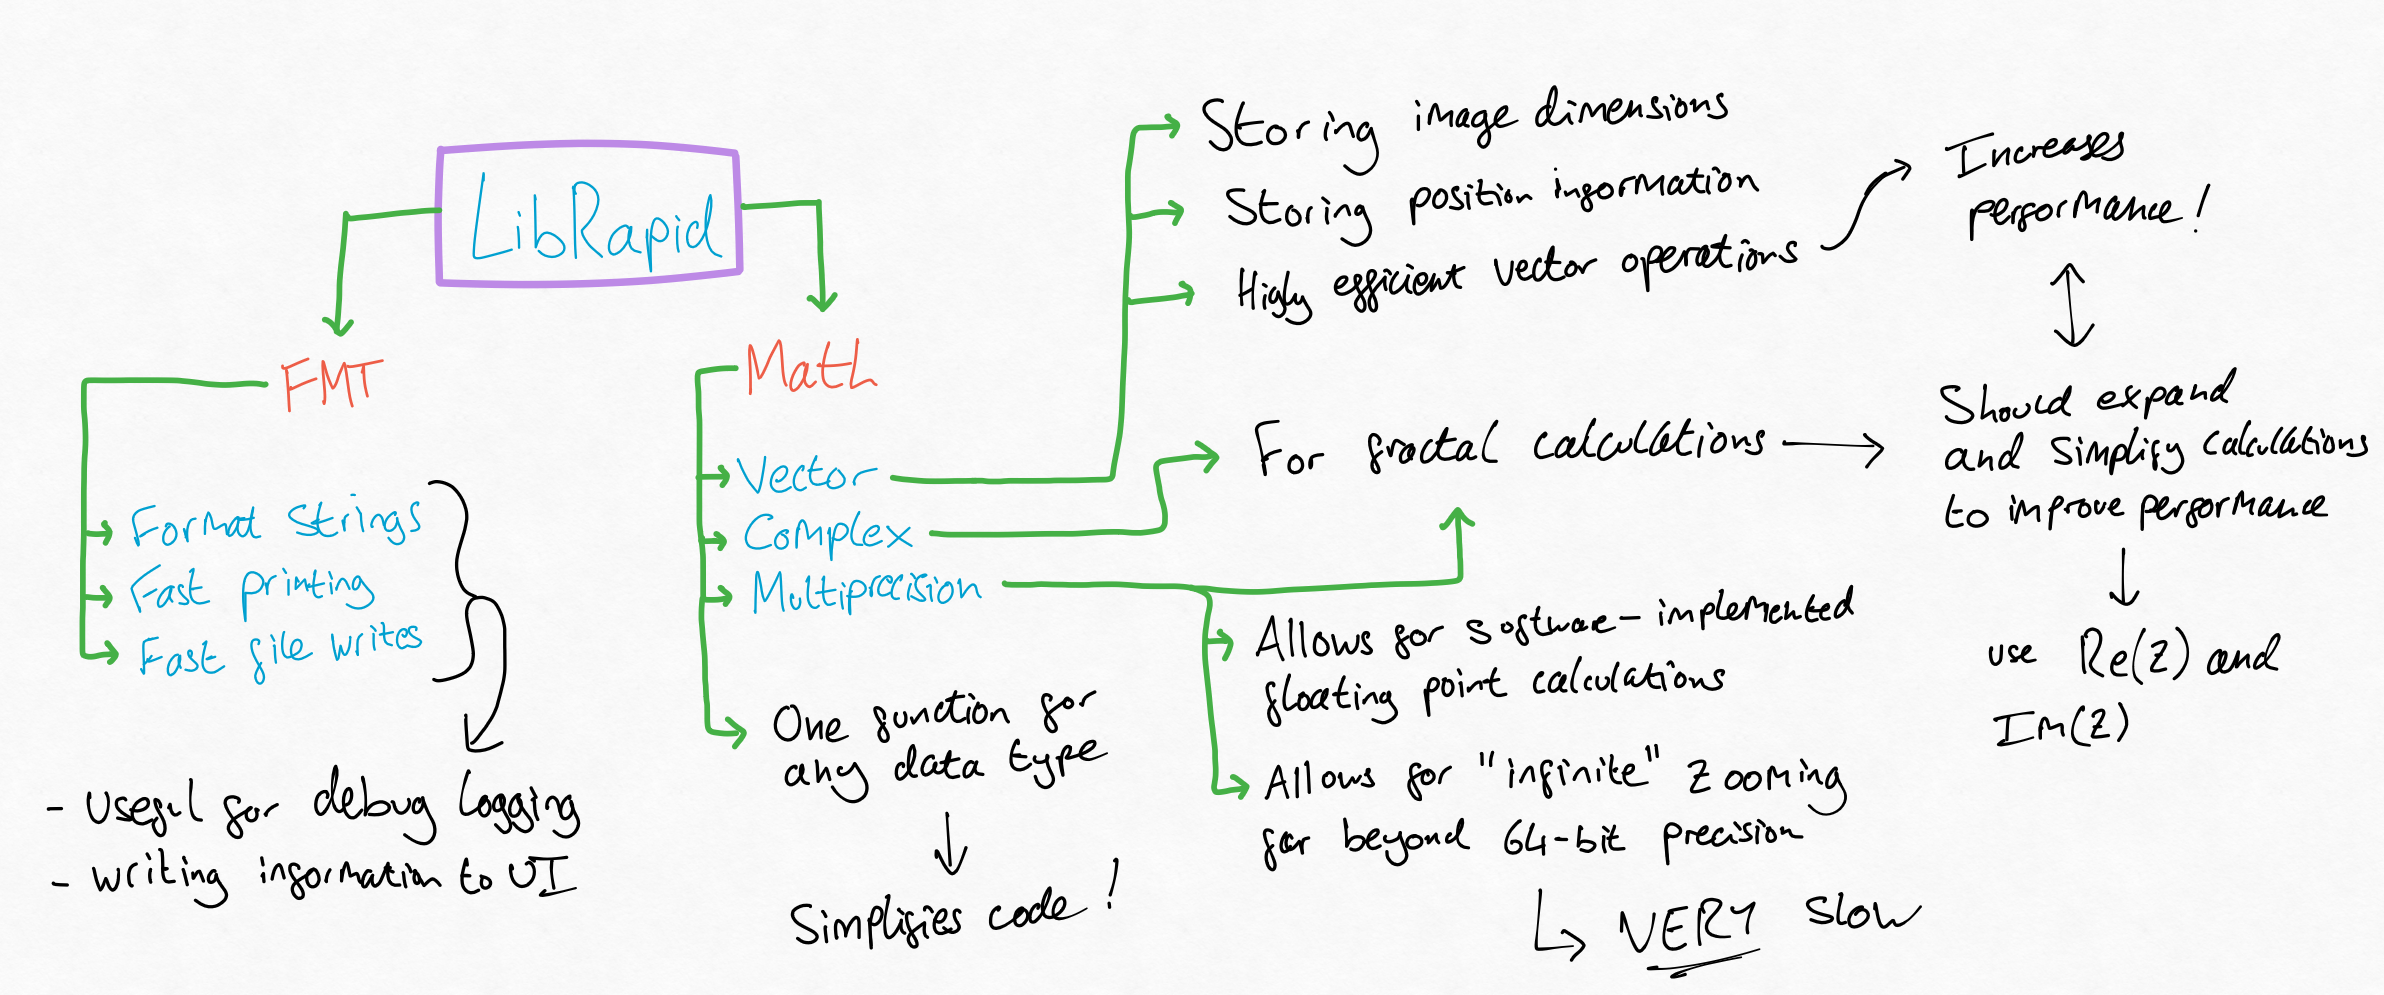
\includegraphics[width=\textwidth]{LibRapidLibraries.png}
	\end{figure*}
\end{center}

\begin{center}
	\begin{figure*}[htp]
		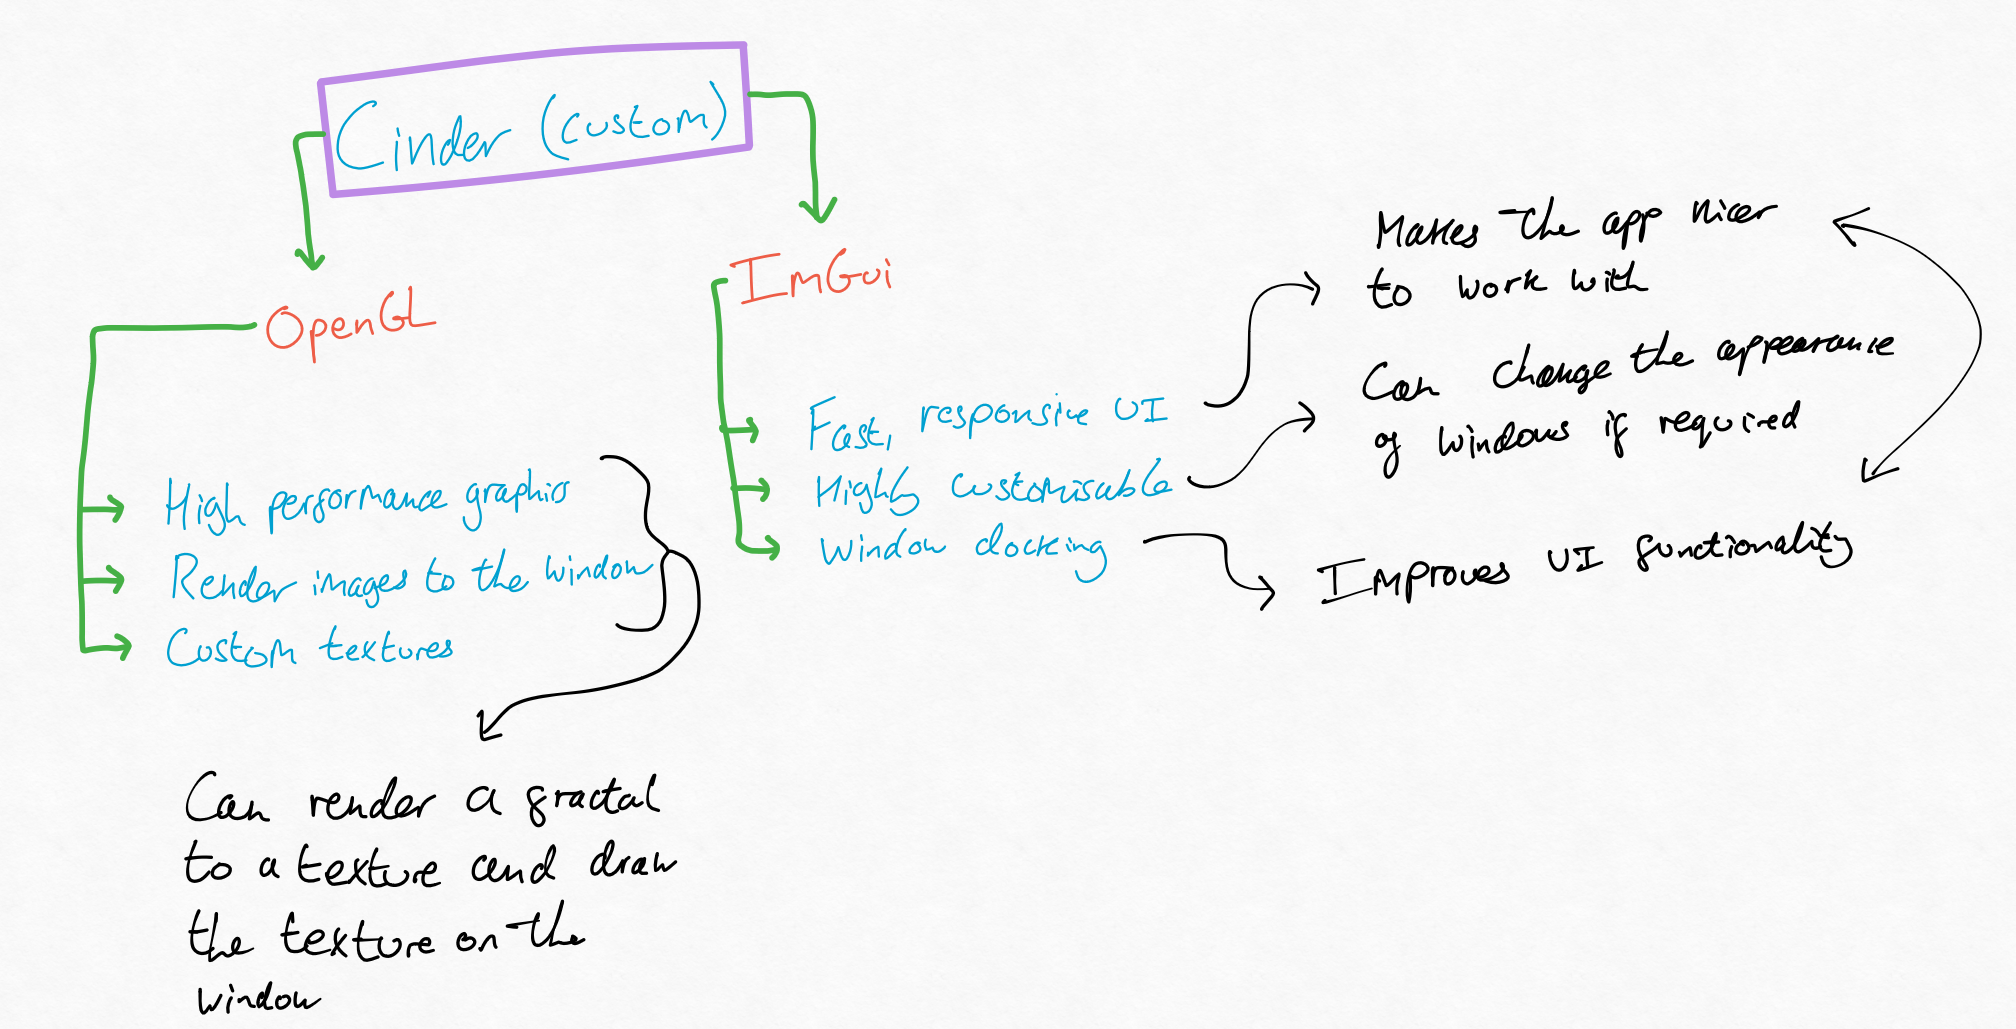
\includegraphics[width=\textwidth]{CinderLibraries.png}
	\end{figure*}
\end{center}

